% TELOS Primacy Attractor and Basin Geometry
% Standalone compilable TikZ diagram
% Compile with: pdflatex fig2_primacy_attractor.tex

\documentclass[border=10pt]{standalone}
\usepackage{tikz}
\usepackage{amsmath}

\begin{document}
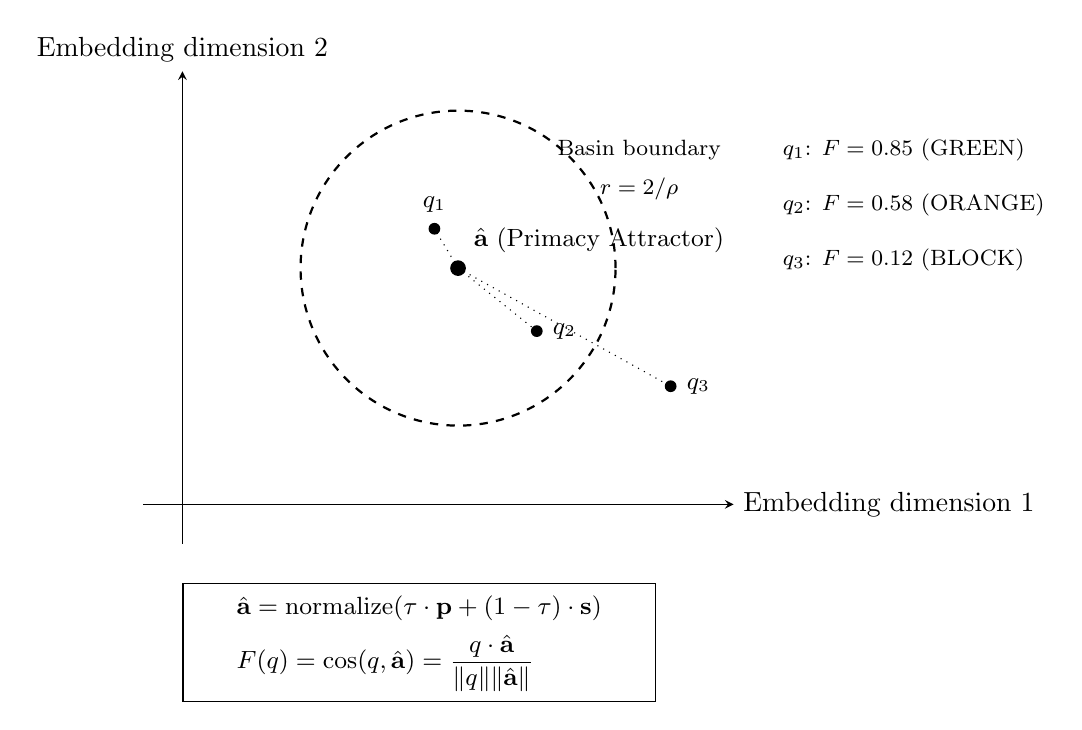
\begin{tikzpicture}[
    >=stealth,
    point/.style={circle, fill=black, inner sep=2pt},
    query/.style={circle, fill=black, inner sep=1.5pt}
]

% Coordinate axes
\draw[->] (-0.5, 0) -- (7, 0) node[right] {Embedding dimension 1};
\draw[->] (0, -0.5) -- (0, 5.5) node[above] {Embedding dimension 2};

% Primacy Attractor point
\coordinate (PA) at (3.5, 3);
\node[point, label={[font=\small]above right:$\hat{\mathbf{a}}$ (Primacy Attractor)}] at (PA) {};

% Basin of attraction (dashed circle)
\draw[dashed, thick] (PA) circle (2cm);
\node[font=\footnotesize] at (5.8, 4.5) {Basin boundary};
\node[font=\footnotesize] at (5.8, 4) {$r = 2/\rho$};

% Query points at different fidelity levels
\coordinate (q1) at (3.2, 3.5);
\coordinate (q2) at (4.5, 2.2);
\coordinate (q3) at (6.2, 1.5);

\node[query, label={[font=\small]above:$q_1$}] at (q1) {};
\node[query, label={[font=\small]right:$q_2$}] at (q2) {};
\node[query, label={[font=\small]right:$q_3$}] at (q3) {};

% Dashed lines from PA to queries (showing fidelity measurement)
\draw[dotted] (PA) -- (q1);
\draw[dotted] (PA) -- (q2);
\draw[dotted] (PA) -- (q3);

% Fidelity annotations
\node[font=\footnotesize, anchor=west] at (7.5, 4.5) {$q_1$: $F = 0.85$ (GREEN)};
\node[font=\footnotesize, anchor=west] at (7.5, 3.8) {$q_2$: $F = 0.58$ (ORANGE)};
\node[font=\footnotesize, anchor=west] at (7.5, 3.1) {$q_3$: $F = 0.12$ (BLOCK)};

% Formula box at bottom
\node[draw, rectangle, minimum width=6cm, minimum height=1.5cm, anchor=north west, font=\small] at (0, -1) {
    \begin{tabular}{l}
    $\hat{\mathbf{a}} = \text{normalize}(\tau \cdot \mathbf{p} + (1-\tau) \cdot \mathbf{s})$\\[4pt]
    $F(q) = \cos(q, \hat{\mathbf{a}}) = \dfrac{q \cdot \hat{\mathbf{a}}}{\|q\| \|\hat{\mathbf{a}}\|}$
    \end{tabular}
};

\end{tikzpicture}
\end{document}
